\chapter{Implémentation et résultats}
\section{Introduction}
Dans le chapitre précédent, nous avons présenté toute la théorie mise en place pour la conception de notre solution de planification de ressources relative à la gestion des ressources dans les environnements Fog. Pour cela, nous avons besoin d'outils nous permettant la quantification des performances et la production de résultat, afin de pouvoir effectuer l'évaluation.\\
Ce chapitre commence par donner un aperçu global sur les différents outils utilisés pour mener à bien la simulation de cette solution, ainsi que les différents éléments ajoutés au simulateur. Enfin nous présentons les résultats en les comparant avec les résultats des différentes politiques gestion classique que sont les politiques : “First fit”, "Best Fit" et "Worst fit".\\

\section{Outil de développement}
Afin de pouvoir simuler la solution proposée, nous avons opté pour le simulateur “IFogSim”. En effet ce dernier opère suivant le paradigme événementiel, ce qui s'accorde parfaitement avec notre solution qui use du même concept. Développé exclusivement en java, IFogSim nous permet de mesurer l'impact technique résultant de la gestion en nous fournissant des données concernant la consommation d'énergie, les délais d'exécution et l'état du réseau.

\subsection{Langage JAVA}
Java est une technologie initialement développée par la société “Sun Microsystems” en 1995, cette dernière s'est vue rachetée par la suite par la société Oracle en 2009. Java fait office à la fois de langage de programmation orienté objet, mais aussi de machine virtuelle qui permet au langage Java d'être multiplateforme. La technologie java bénéficie d'une grande popularité dû aux avantages considérables proposés par cette dernière parmi lesquels :
\begin{itemize}
    \item La portabilité : i.e la capacité du même code java à s'exécuter sur plusieurs systèmes d'exploitation.
    %\item Popularité
    \item Richesses des bibliothèques disponibles
    \item Gratuité 
\end{itemize}

\subsection{L'outil IFogSim}
IFogSim est un outil de modélisation d'environnements Cloud-Fog-IoT créé par
Harshit Gupta (chef de projet) au Georgia Institute of Technology, Atlanta, GA, USA dans l'objectif de simuler l'impact des différentes techniques du management des ressources sur les environnements Fog. IFogSim mesure l'impact d'une politique sur un système par sa latence, l'utilisation de la bande passante, la consommation d'énergie et l'utilisation des ressources des nœuds. IFogSim a été conçu en tant qu'extension à l'outil CloudSim, qui est un simulateur Open Source d'applications Cloud développé en Java. IFogSim est donc lui aussi Open Source et programmé en Java .

\subsection{Architecture de l'IFogSim}
L'iFogSim est composé de 3 composants principaux, à savoir : 
\begin{itemize}
    \item Les composants physiques.
    \item Les composants logiques.
    \item Les composants de gestion.
\end{itemize}

\subsubsection{Composants physiques}
Les composants physiques incluent le cloud, les nœuds Fog et les objets, qui sont organisés dans un ordre hiérarchique. Les noeuds Fog de niveau inférieur sont directement connectés aux capteurs et actionneurs associés. Les noeuds Fog agissent comme des centres de traitement de données en offrant de la mémoire et de la puissance de calcul. Chaque noeud Fog est créé avec une puissance de calcul et des attributs de consommation d'énergie spécifique (puissance occupée et inactive), qui reflètent ses capacités et son efficacité énergétique. Les capteurs génèrent des tuples qui peuvent être appelés tâches dans le cloud computing. La création de tuples (tâches) est pilotée par les événements et l'intervalle entre la génération de deux tuples est régi par une distribution déterministe définie lors de la création des capteurs.

\subsubsection{Composants logiques}
Les modules d'application (AppModules) et les bords d'application (AppEdges) sont les composants logiques d'IFogSim. Dans IFogSim, une application est considérée comme une collection des modules interdépendants, ce qui améliore par conséquent le concept d'application distribuée. La dépendance entre deux modules est définie par les fonctionnalités d'AppEdges qui sont le flux de données logique entre deux modules d'application. Dans iFogSim, chaque module d'application (AppModule) traite un type particulier de tâche (tuple). La transmission de tuples entre deux modules d'application (AppModules) peut être périodique.

\subsubsection{Composants de gestion}
Les composants de gestion d'IFogSim sont représentés par le « Controller» et le «ModuleMapping». Selon les exigences des AppModules, l'objet ModuleMapping identifie les noeuds fog associés à chaque AppModules. L'objet Controller lance les AppModules sur leurs noeuds Fog attribués en suivant les informations de placement fournies par l'objet ModuleMapping, et gère périodiquement les ressources des noeuds Fog. Une fois la simulation terminée, l'objet Controller collecte les résultats des coûts, de l'utilisation du réseau et de la consommation d'énergie pendant la période de simulation à partir des noeuds Fog.
\begin{figure}[H]
    \centering
    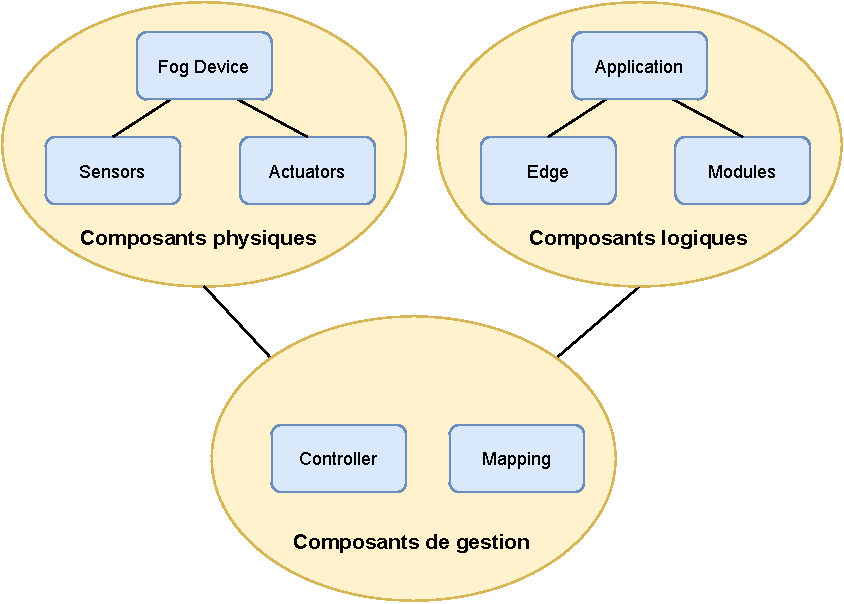
\includegraphics[]{Diagramme d'interaction.pdf}
    \caption{Diagramme représentant l'interaction des différents composants de l'IFogSim}
    % \label{fig:}
\end{figure}

\subsubsection{Description des classes principales}
Les principales classes de l'IFogSim sont les suivantes :
\begin{itemize}
    \item \textbf{\emph{FogDevice :}} Cette classe spécifie les caractéristiques matérielles des nœuds Fog et leurs connexions aux autres nœuds de la topologie. Les principaux attributs de cette classe sont la mémoire accessible, le processeur, la taille de stockage, la bande passante de la liaison montante et la liaison descendante. Les méthodes de cette classe définissent la manière dont les ressources d'un nœud Fog sont planifiées entre les modules qui s'exécutent sur cette application, ainsi que leur déploiement. Par défaut, chaque FogDevice ne peut avoir hiérarchiquement qu'un seul père.
    \item \textbf{\emph{Sensor :}}  les instances de la classe Sensor sont des entités qui agissent en tant que capteurs IoT tels que décrits dans l'architecture. La classe contient des attributs représentant les caractéristiques d'un capteur (son nom, le tuple d'émission et un paramètre qui représente les conditions d'émission du Tuple). La classe contient un attribut de référence au dispositif Fog auquel le capteur est connecté et la latence de connexion entre eux. 
    \item \textbf{\item{Actuator  :}} -  Cette classe modélise un actionneur en définissant l'effet de l'actionnement et ses propriétés de connexion au réseau. La classe définit une méthode pour effectuer une action à l'arrivée d'un tuple à partir d'un module d'application. Un attribut de la classe fait référence à la passerelle à laquelle l'actionneur est connecté et à la latence de cette connexion.
    \item \textbf{\item{Tuple :}} Les tuples forment l'unité fondamentale de communication entre les entités dans le réseau Fog. Il peut être soit une tâche, soit une donnée. Un tuple est caractérisé par son type, sa source et sa destination. Les attributs de la classe spécifient la puissance de calcul nécessaire à son traitement (mesuré en millions d'instructions (MI)) et la longueur des données encapsulées dans le tuple.
    \item \textbf{\item{Application :}} Les instances de cette classe représentent les éléments qui composent une application. Pour chaque tuple entrant, une instance AppModule le traite et génère des tuples en sortie, qui sont envoyés aux modules suivants. Le nombre de tuples de sortie par tuple d'entrée est déterminé à l'aide d'un modèle de sélectivité, qui peut être basé sur une sélectivité fractionnaire ou un modèle éclaté.
    \begin{itemize}
        \item \textbf{\emph{AppEdge :}} Une instance AppEdge dénote la dépendance entre une paire de modules d'application. Chaque AppEdge est caractérisé par le type de tuple qu'il transporte, les exigences de traitement et la longueur des données encapsulées dans ces tuples. l'IFogSim prend en charge deux types d' AppEdge (périodique et événementiels). Les tuples dans les AppEdge périodiques sont émis à intervalles réguliers. Le tuple dans un AppEdge est basé sur un événement qui est envoyé lorsque le module source reçoit un tuple précis.
        \item \textbf{\emph{AppLoop :}} est une classe supplémentaire, utilisée pour spécifier les boucles de contrôle de processus qui intéressent l'utilisateur. Dans l'IFogSim, le développeur peut spécifier les boucles de contrôle pour mesurer la latence de bout en bout. Une instance AppLoop est fondamentalement une liste de modules à partir de l'origine de la boucle jusqu'au module où la boucle se termine.
    \end{itemize}
    \item \textbf{\emph{Config :}} Cette classe abstraite a pour but de contenir tous les paramètres qui affectent la simulation par exemple MAX\_SIMULATION\_TIME qui représente la durée de simulation.
    \item \textbf{\emph{Controller :}} cet objet se charge d'orchestrer la simulation. Concrètement, il sert à initialiser la topologie avant le début de la simulation, ainsi qu'à effectuer les traitements de fin de simulation (notamment afficher et exporter les résultats).
\end{itemize}
\begin{figure}[H]
    \centering
    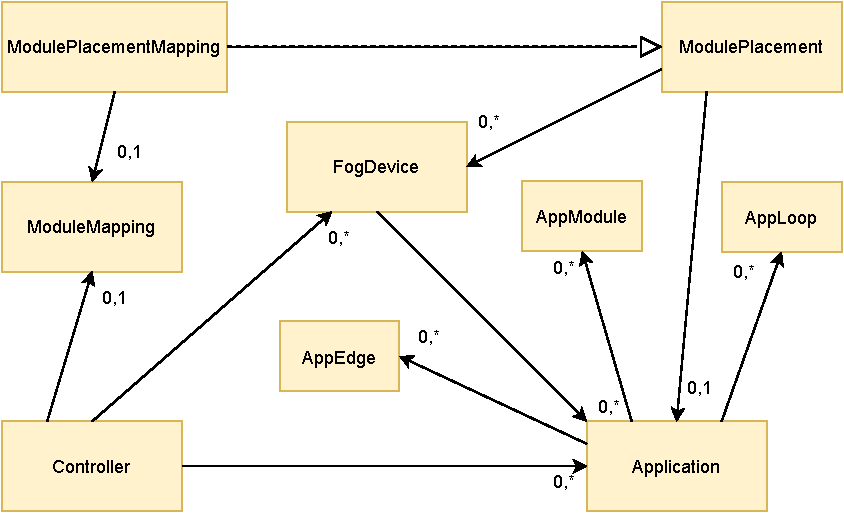
\includegraphics[]{Diagramme de relation.pdf}
    \caption{Diagramme représentant les relations entre les principales classes de l'IFogSim}
    % \label{fig:}
\end{figure}

\section{Développement de la conception}
Afin de mettre en œuvre la conception proposée, nous allons ajouter de nouvelles classes nécessaires à l'implémentation de la solution, mais aussi la modification de certaines classes principales de l'IFogSim afin de l'adapter à nos besoins.\\
Les manipulations effectuées pour mettre en oeuvre cette solution sont énumérées ci-dessous : 
\begin{enumerate}
    \item \textbf{Création d'une classe ClusterFogDevice :} Cette classe représente un nœud Fog quelconque du cluster. Elle étend la classe prédéfinie FogDevice et comporte en plus les attributs suivant:
\begin{itemize}
    \item \textbf{parentsIds :} qui est une liste qui contient les identificateurs des nœuds se trouvant au niveau supérieur.
    \item \textbf{isNorthLinkBusyById :} qui est une liste de booléens où chaque élément indique si la liaison supérieure en question est occupée.
    \item \textbf{northTupleQueues :} qui est une liste de files d'attente de tuple qui associe à chaque liaison supérieure une file de tuples où seront stockés les tuples à envoyer sur cette liaison si cette dernière est occupée.
\end{itemize}
De plus, la méthode  processTupleArrival, qui est la méthode exécutée par le noeud à chaque arrivée d'un tuple, a été redéfinie afin d'implémenter la routine associée à un noeud fog et qui est décrite dans la conception.
     \item \textbf{Création d'une classe GWFogDevice :} cette classe représente un nœud Fog passerelle, c.-à-d. le noeud connecté directement aux capteurs et aux actionneurs. Cette classe étend également la classe FogDevice, et ajoute les attributs suivants :
     \begin{itemize}
     \item \textbf{waitingQueue :} qui est une liste de tuples servant à stocker les demandes non encore affectées.
     \item \textbf{tupleToMatchedDevice :} est une liste contenant les tuples non affectés à un neud.
     \item \textbf{matchedTupleList :} qui est une liste comportant les tuples affectés à leurs nœuds respectifs.
     \item \textbf{gwDevices :} est une liste de GWFogDevice, contenant l'ensemble de nœuds passerelles.
     \item \textbf{isNorthLinkBusyById :} qui représente la même chose que dans la classe.
     \item \textbf{northTupleQueues :} elle représente également la même chose que celle mentionnée dans la classe ClusterFogDevice.
     \item \textbf{clusterFogDevicesIds :} qui représente la liste de tous les noeuds Fog du cluster.
     \end{itemize}
     \item \textbf{Création d'une classe MatchedTuple :} cette classe décrit les tuples une fois affectés à leurs noeuds respectifs. Elle représente un enrichissement de la classe Tuple par les attributs suivants :
     \begin{itemize}
         \item \textbf{destinationFogDeviceId :} qui contient l'identificateur du noeud de destination.
         \item \textbf{destModuleMips :} qui décrit les exigences de traitement du module de destination.
     \end{itemize}
\end{enumerate}
La même procédure à été effectueé pour implémenter les politiques concurrentes.

\section{Résultats et évaluation des performances :}
Afin de pouvoir juger des performances ainsi que l'ampleur des gains apportés par notre modèle de planification de ressources, nous évaluons les performances de cette solution en mesurant le délai d'exécution des applications, et le délai d'exécution des tuples. Puis nous comparons les résultats avec des modèles classiques implémentant les stratégies “FirstFit”,"BestFit","WorstFit".\par
Les nœuds fog ainsi que les demandes générées sont créés avec une certaine hétérogénéité permettant de mieux étudier la capacité de notre algorithme à faire correspondre une variété de demandes à des nœuds avec de différentes capacités matérielles.\par
Les résultats sont représentés par les graphes suivants (les résultats sont normalisés par rapport à la valeur maximale, donc sur une échelle de 0 à 1) :

\subsubsection{Scalabilité verticale}
Nous mesurons dans cette partie les performances du modèle par rapport à la variation du nombre de niveaux de la matrice \emph{Fog} précédemment définie.

\begin{figure}[H]
  \centering
  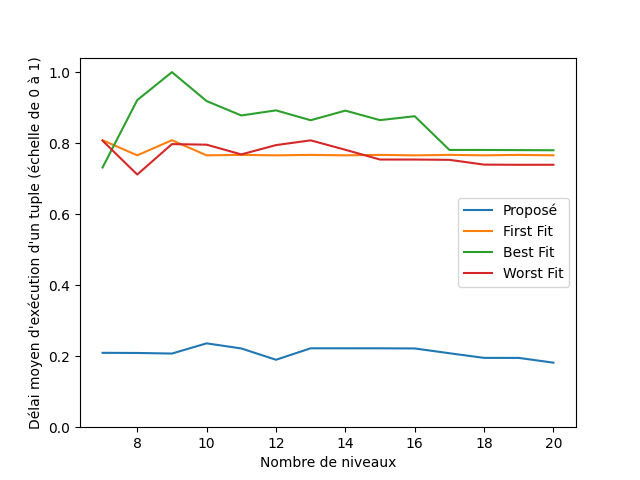
\includegraphics[]{resultats/tupleDelayV.png}
  \caption{Délai moyen d'exécution d'un tuple en fonction du nombre de nivaux}
  \label{fig:delai_tuple_vertical}
\end{figure}

\begin{figure}[H]
  \centering
  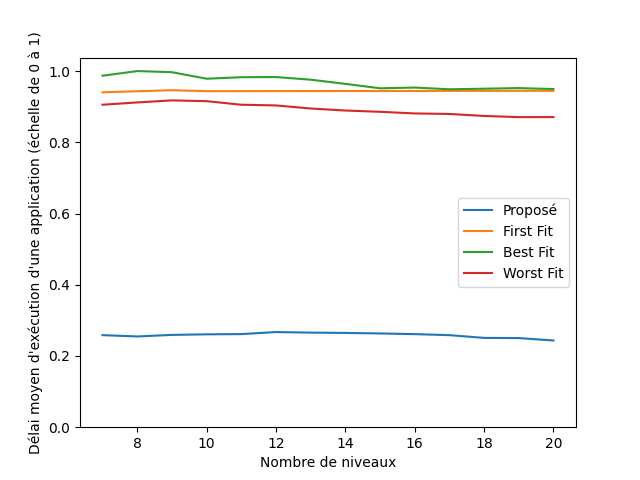
\includegraphics[]{resultats/loopDelayV.png}
  \caption{Délai moyen d'exécution d'une application en fonction du nombre de nivaux}
  \label{fig:delai_application_vertical}
\end{figure}

Les figures \ref{fig:delai_tuple_vertical} et \ref{fig:delai_application_vertical} montrent, respectivement, la variation du délai moyen de l'exécution d'un tuple (représentant une demande de service) et le délai d'exécution d'une application complète selon la nombre de niveaux de l'architecture.\par
Nous constatons une nette réduction du délai de traitement des tuples d'environ 75\%, en comparaison aux reste des algorithmes de la simulation. Cette réduction se stabilise au-delà du seuil de 18 niveaux, où le nombre de niveaux n'influence plus cette métrique. De même pour le délai d'exécution d'une application, où nous pouvons constater l'impact de la réduction du temps de réponse des tuples individuels.

\subsubsection{Scalabilité horizontale}
Nous mesurons dans cette partie les performances du modèle par rapport à la variation du nombre de nœuds par niveau de la matrice \emph{Fog} précédemment définie.\par
Le nombre de nœuds par niveau influence le nombre de tuples générés par les objets IoT car chaque nœud passerelle est relié à un ensemble d’objets IoT. Ainsi l’augmentation du nombre de nœuds passerelle augmente aussi le nombre de demandes générées.

\begin{figure}[H]
  \centering
  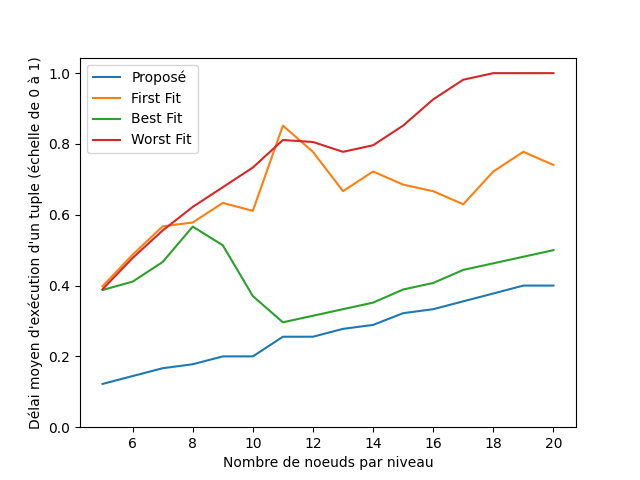
\includegraphics[]{resultats/tupleDelayH.png}
  \caption{Délai moyen d'exécution d'un tuple en fonction du nombre de nœuds par nivaux}
  \label{fig:delai_tuple_horizontal}
\end{figure}

\begin{figure}[H]
  \centering
  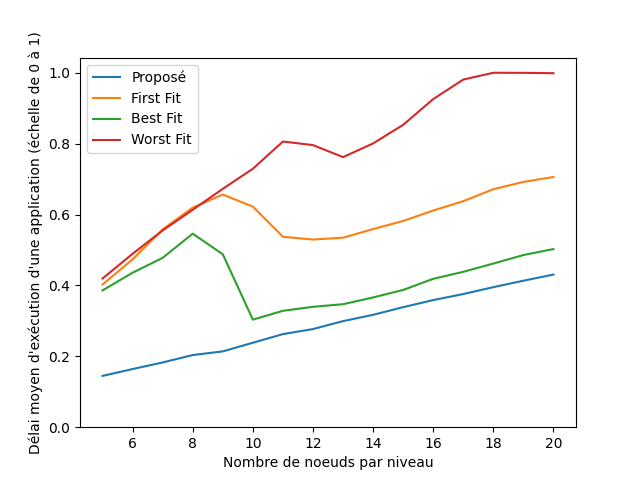
\includegraphics[]{resultats/loopDelayH.png}
  \caption{Délai moyen d'exécution d'une application en fonction du nombre de nœuds par niveau}
  \label{fig:delai_application_horizontal}
\end{figure}

Les figures \ref{fig:delai_tuple_horizontal} et \ref{fig:delai_application_horizontal} représentent, respectivement, la variation du délai de l'exécution d'un tuple et le délai d'exécution d'une application selon le nombre de nœuds par niveau.\par
La figure \ref{fig:delai_tuple_horizontal} montre un délai d'exécution croissant linéairement de la part des stratégies classiques, contrairement à la méthode proposée qui semble suivre une tendance logarithmique. Nous concluons par conséquent que pour les stratégies classiques, l'augmentation du nombre de nœuds par niveau influe significativement sur le délai d'exécution d'une application, par opposition à la stratégie proposée ou la corrélation semble moins significative.\par
Nous remarquons que pour la stratégie "Best Fit", la croissance de la duré d'exécution d'un tuple est linéairement croissante en fonction du nombre de nœuds par niveau. Pour la stratégie "First Fit", la durée d'exécution augmente jusqu'à se stabiliser quand le nombre de nœuds dépasse 19 nœuds par niveau. Ainsi que pour la stratégie "Worst Fit", nous constatons une augmentation suivie d'une phase de diminution à partir de 17 nœuds par nivaux. Enfin la stratégie proposée semble suivre une cadence doucement haussière en ayant de meilleurs résultats, ainsi qu'une meilleure stabilité du temps d'exécution.

\subsubsection{Étude selon le débit des demandes}
Dans ce qui suit, nous étudions les performances de notre modèle selon le délai entre l'envoi de chaque demande. Naturellement, plus le délai entre les demandes est petit, plus il y a de charge et de congestion dans le réseau.

\begin{figure}[H]
  \centering
  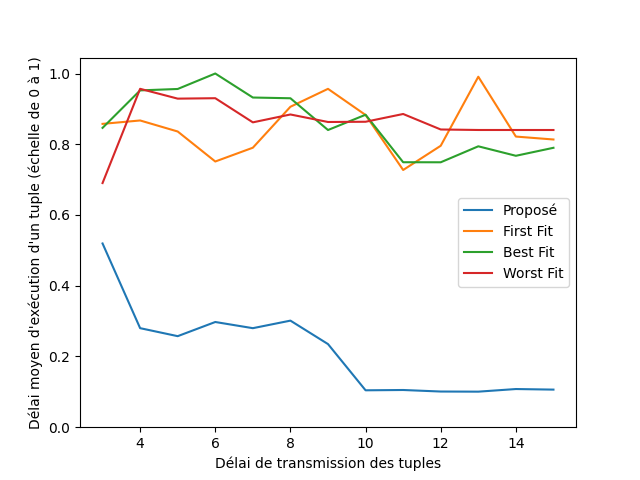
\includegraphics[]{resultats/tupleDelayT.png}
  \caption{Délai moyen d'exécution d'un tuple en fonction du taux de transmission}
  \label{fig:delai_tuple_debit}
\end{figure}

\begin{figure}[H]
  \centering
  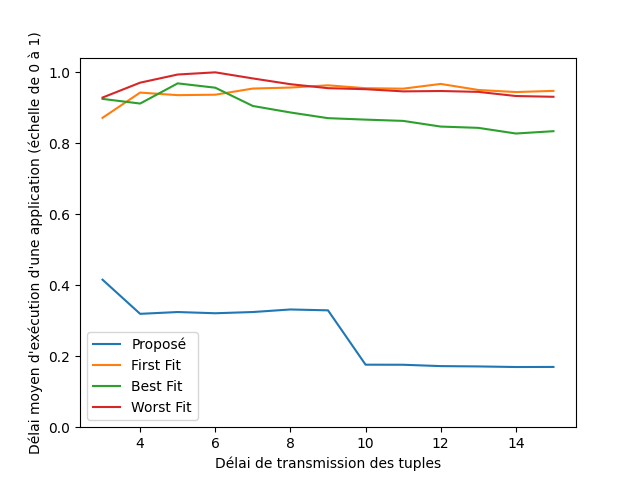
\includegraphics[]{resultats/loopDelayT.png}
  \caption{Délai moyen d'exécution d'une application en fonction du taux de transmission}
  \label{fig:delai_application_debit}
\end{figure}

Les figures \ref{fig:delai_tuple_debit} et \ref{fig:delai_application_debit} représentent, respectivement, la variation du délai d'exécution d'un tuple et le délai d'exécution d'une application selon le délai de transmission entres les tuples consécutifs.
Nous constatons que la durée d'exécution d'une application dans les stratégies classique est stable et proche de la valeur maximale, ce qui signifie que la diminution de la charge de travail, n'influe pas sur la dure d'exécution. En revanche, la stratégie proposée démontre des performances meilleures en termes de délai ainsi qu'une réaction à la variation du délai de transmission à partir de 9 unités de délai.\par

\section{Conclusion}
Nous avons réussi à montrer l'efficacité de notre technique dans la réduction du temps d'exécution des demandes de services, témoignant ainsi d'une distribution équitable et efficace des charges de travail sur l'ensemble des nœuds du cluster. Cette technique permet aussi de minimiser l'interaction des objets IoT avec le Cloud et le coût du trafic réseau engendré.